% Provenance (never printed): see sources/outline_sources.md (Year 1: rigid plates on a
% sphere, Euler poles and angular velocities; relative velocities; triple junctions;
% finite rotations; the magnetic-anomaly timescale; satellite geodesy). Curves and maps
% from figdata/bachelor-1/euler_velocities.py, south_atlantic_fit.py and gpts_stripes.py;
% exercise and problem values in the Book 3 scratch calculator calc/ch12.py.
\chapter{Cinemática de placas sobre uma esfera}\label{ch:b1:plate-kinematics}

Duas estações de posicionamento por satélite vêm registrando suas posições todos os dias há mais de um quarto de século: uma em Reykjavik, no oeste da Islândia, a outra perto de Stavanger, na costa oeste da Noruega. A linha reta entre elas, de \qty{1546}{km}, cresce \qty{17.5}{mm} a cada ano, quase dois centímetros. Nada no terreno mostra isso, e o fundo do Atlântico Norte entre as duas estações registra o mesmo alargamento há milhões de anos: a lava erupcionada na Dorsal Meso-Atlântica adquiriu a direção do campo magnético terrestre ao esfriar, e o campo já se inverteu muitas vezes, de modo que o fundo oceânico carrega um registro listrado de seu próprio crescimento. Este capítulo transforma as placas dos anos escolares em calotas rígidas sobre uma esfera, descreve seus movimentos com a geometria das rotações, e mostra como o registro geológico e os satélites medem os mesmos movimentos.
% ledger: ngl:reyk, ngl:stas (chord lengthening computed in calc/ch12.py)

\begin{recall}
Numa esfera, um \omterm{def:b1:spherical-astronomy:spherical-triangle}{círculo máximo} é a interseção com um plano que passa pelo centro; um \omterm{def:b1:spherical-astronomy:spherical-triangle}{círculo menor}, com qualquer outro plano. A lei dos cossenos dá a distância angular entre dois pontos a partir de suas \omterm{def:b1:spherical-astronomy:geographic}{latitudes} e \omterm{def:b1:spherical-astronomy:geographic}{longitudes}, e o \omterm{def:b1:spherical-astronomy:horizontal}{azimute} de uma \omterm{def:b1:geological-maps:attitude}{direção} é contado a partir do norte, para leste
(\cref{ch:b1:spherical-astronomy}). Um corpo rígido que gira em torno de um eixo fixo tem uma velocidade angular (física). A \omterm{def:b1:layered-earth:lithosphere}{litosfera} está quebrada em placas que se movem umas em relação às outras a alguns centímetros por ano, e o fundo oceânico
carrega listras magnéticas que registram as inversões do campo magnético terrestre (Livro 2, 11º ano).
\end{recall}

\section{Placas rígidas sobre uma esfera}

Uma placa cobre uma grande parte da esfera: a placa euroasiática se estende do meio do Atlântico até a Sibéria oriental. Seu movimento não pode ser descrito por uma velocidade, como o movimento de um carro; ele deve ser descrito por uma rotação.

\begin{definition}[Placa rígida]\label{def:b1:plate-kinematics:rigid-plate}
A \emph{placa rígida}\index{placa rígida} é uma região da \omterm{def:b1:layered-earth:lithosphere}{litosfera} cujo
interior não se deforma de modo mensurável: a distância entre quaisquer dois de seus pontos
permanece constante. O movimento relativo de duas placas é absorvido ao longo de sua
fronteira comum, uma zona estreita de falhas, terremotos e vulcões.
\end{definition}

Nenhuma placa é perfeitamente rígida: as fronteiras são zonas de dezenas a centenas de quilômetros de largura, e os interiores se deformam lentamente. A hipótese é que esses desvios são pequenos diante dos movimentos relativos; ela é testada pela consistência de cada resultado deste capítulo.

Uma \omterm{def:b1:plate-kinematics:rigid-plate}{placa rígida} na superfície de uma esfera se move sem mudar a distância entre quaisquer dois de seus pontos, e o centro da Terra não se move. Tal movimento é descrito
por uma matriz $3\times3$ $R$ que conserva comprimentos, uma matriz \emph{ortogonal} ($R^{\mathsf T}R = I$), e que conserva a orientação do espaço, de modo que $\det R = 1$:
um ponto de vetor posição $\vec r$ vai para $R\vec r$.

\begin{theorem}[Teorema da rotação de Euler]\label{thm:b1:plate-kinematics:euler}
Todo deslocamento de uma \omterm{def:b1:plate-kinematics:rigid-plate}{placa rígida} na esfera é uma rotação em torno de um eixo
que passa pelo centro da Terra: existe um vetor unitário $\vec n$ com
$R\vec n = \vec n$, e a placa gira em torno de $\vec n$ de algum ângulo.
\end{theorem}

\begin{proof}
Mostramos que $1$ é um autovalor de $R$, isto é $\det(R - I) = 0$. Como
$R R^{\mathsf T} = I$, temos $R - I = R(I - R^{\mathsf T})$, logo
\[
  \det(R - I) = \det R\,\det\bigl((I - R)^{\mathsf T}\bigr) = \det(I - R),
\]
usando $\det R = 1$ e o fato de que uma matriz e sua transposta têm o mesmo
determinante. Para uma matriz $3\times3$,
$\det(I - R) = (-1)^3\det(R - I) = -\det(R - I)$. Logo $\det(R - I) =
-\det(R - I)$, que é nulo. Existe portanto um vetor unitário $\vec n$ com $R\vec n = \vec n$:
os dois pontos em que a reta pelo centro ao longo de $\vec n$ encontra a superfície
não se movem. No plano perpendicular a $\vec n$, $R$ conserva comprimentos e orientação:
ele gira esse plano de algum ângulo, e assim gira a esfera inteira em torno de $\vec n$.
\end{proof}

Em um intervalo de tempo curto o bastante para que o movimento não mude, a
rotação se dá a uma taxa constante, e o movimento de uma placa em relação a
outra é uma velocidade angular em torno de um eixo fixo.

\begin{definition}[Polo de Euler; vetor de Euler]\label{def:b1:plate-kinematics:euler-pole}
O movimento de uma placa B em relação a uma placa A é uma rotação em torno de um eixo
que passa pelo centro da Terra. O \emph{polo de Euler}\index{polo de Euler} do par é o ponto em que esse eixo encontra a superfície, escolhido de modo que a
rotação seja anti-horária vista de cima dele; o ponto antípoda é o
polo oposto. O \emph{vetor de Euler}\index{vetor de Euler}
$\vec\omega_{BA}$ é a velocidade angular de B em relação a A: ele aponta do centro da Terra para o polo de Euler, e seu comprimento $\omega$ é a
taxa de rotação.
\end{definition}

Um \omterm{def:b1:plate-kinematics:euler-pole}{vetor de Euler} é dado pela \omterm{def:b1:spherical-astronomy:geographic}{latitude} e \omterm{def:b1:spherical-astronomy:geographic}{longitude} de seu polo e por sua
taxa, em geral em graus por milhão de anos. O movimento da placa euroasiática
em relação à placa norte-americana, média dos últimos \qty{3.16}{Myr}
a partir de 453 taxas de espalhamento medidas nas dorsais entre elas, tem seu polo em
\ang{61.8}\,N, \ang{139.6}\,L, na Sibéria oriental, e a taxa
\qty{0.210}{\degree\per\Myr}. Em radianos por ano,
\[
  \omega = \frac{0.210\times\pi/180}{\num{e6}} = \qty{3.665e-9}{rad.yr^{-1}},
\]
uma volta completa em \qty{1714}{\Myr}.
% ledger: morvel:eu-na, morvel:summary

\section{Velocidades relativas}

\begin{theorem}[Velocidade em uma placa em rotação]\label{thm:b1:plate-kinematics:velocity}
Se a placa B gira em relação à placa A com o \omterm{def:b1:plate-kinematics:euler-pole}{vetor de Euler} $\vec\omega$, um ponto
de B de vetor posição $\vec r$ (a partir do centro da Terra) se move
em relação a A com a velocidade
\[
  \vec v = \vec\omega\times\vec r .
\]
\end{theorem}

\begin{proof}
Seja $\Delta$ o ângulo entre $\vec\omega$ e $\vec r$. Ao girar, B faz o ponto descrever um círculo em torno do eixo, de raio $R\sin\Delta$, onde $R$ é o raio da Terra; à taxa angular $\omega$, sua velocidade é
$\omega R\sin\Delta$. Sua velocidade é tangente a esse círculo, logo perpendicular ao eixo e ao raio $\vec r$, e, sendo a rotação anti-horária em torno de $\vec\omega$, seu sentido é o de $\vec\omega\times\vec r$.
O vetor $\vec\omega\times\vec r$ tem precisamente esta direção e este sentido, e
o comprimento $\omega R\sin\Delta$.
\end{proof}

O ângulo $\Delta$ é a distância angular entre o \omterm{def:b1:plate-kinematics:euler-pole}{polo de Euler} e o ponto,
que a lei dos cossenos dá a partir de \omterm{def:b1:spherical-astronomy:geographic}{latitudes} e \omterm{def:b1:spherical-astronomy:geographic}{longitudes}.

\begin{proposition}[Velocidade e direção do movimento relativo]\label{prop:b1:plate-kinematics:speed}
Seja o \omterm{def:b1:plate-kinematics:euler-pole}{polo de Euler} na \omterm{def:b1:spherical-astronomy:geographic}{latitude} $\varphi_p$ e \omterm{def:b1:spherical-astronomy:geographic}{longitude} $\lambda_p$, e o ponto em $\varphi$ e $\lambda$. Então
\begin{enumerate}
  \item a distância angular $\Delta$ do polo ao ponto satisfaz
        $\cos\Delta = \sin\varphi_p\sin\varphi + \cos\varphi_p\cos\varphi
        \cos(\lambda - \lambda_p)$;
  \item a velocidade relativa é $v = \omega R\sin\Delta$: nula no polo,
        máxima, $\omega R$, no \omterm{def:b1:spherical-astronomy:spherical-triangle}{círculo máximo} a \ang{90} dele;
  \item a direção do movimento é perpendicular ao \omterm{def:b1:spherical-astronomy:spherical-triangle}{círculo máximo} que une o
        ponto ao polo: seu \omterm{def:b1:spherical-astronomy:horizontal}{azimute} é o do polo, visto do ponto,
        mais \ang{90}.
\end{enumerate}
\end{proposition}

\begin{proof}
(1) é a lei dos cossenos no \omterm{def:b1:spherical-astronomy:spherical-triangle}{triângulo esférico} formado pelo polo norte geográfico, o \omterm{def:b1:plate-kinematics:euler-pole}{polo de Euler} e o ponto, cujos lados a partir do polo norte são
$\ang{90} - \varphi_p$ e $\ang{90} - \varphi$, com o ângulo
$\lambda - \lambda_p$ entre eles. (2) segue do teorema. (3) A
velocidade é perpendicular a $\vec\omega$ e a $\vec r$, logo ao plano que os contém, o plano do \omterm{def:b1:spherical-astronomy:spherical-triangle}{círculo máximo} que passa pelo ponto e pelo polo. No
plano horizontal no ponto, ela é portanto perpendicular à direção do polo; sendo a rotação anti-horária vista de cima do
polo, um ponto se move à direita da direção em que vê o polo, o que acrescenta \ang{90} ao \omterm{def:b1:spherical-astronomy:horizontal}{azimute}.
\end{proof}

\begin{omfigure}
\begin{tikzpicture}[x=2.5cm, y=2.5cm, font=\scriptsize, >=Stealth]
% orthographic view from 20 deg above the "Euler equator": a point at polar angle D,
% longitude p about the pole projects to X = sin D sin p, Y = cos D cos 20 - sin D cos p sin 20;
% it is visible when cos p >= -cot D tan 20 (limits computed by hand: 129.08, 102.13, 90, 77.87)
\fill[omSea!12] (0,0) circle (1);
\draw[thick] (0,0) circle (1);
\foreach \D/\m in {30/129.08, 60/102.13, 90/90, 120/77.87} {
  \draw[blue!45!black, domain=-\m:\m, samples=60, variable=\p]
    plot ({sin(\D)*sin(\p)}, {cos(\D)*cos(20) - sin(\D)*cos(\p)*sin(20)});
  \draw[blue!45!black, densely dashed, domain=\m:360-\m, samples=60, variable=\p]
    plot ({sin(\D)*sin(\p)}, {cos(\D)*cos(20) - sin(\D)*cos(\p)*sin(20)});
}
\draw[densely dashed] (0,0) -- (0,0.9397);
\draw[->, very thick] (0,0.9397) -- (0,1.38) node[above] {$\vec\omega$};
\fill (0,0.9397) circle (0.9pt) node[anchor=south west] {polo de Euler};
\fill (0,0) circle (0.7pt);
% velocity arrows at longitude -35 deg about the pole, length 0.5 sin D
\draw[->, very thick, red!75!black] (-0.287,0.6737) -- ++(0.243,-0.058);
\draw[->, very thick, red!75!black] (-0.497,0.2272) -- ++(0.421,-0.101);
\draw[->, very thick, red!75!black] (-0.574,-0.2802) -- ++(0.487,-0.117);
\draw[->, very thick, red!75!black] (-0.497,-0.7124) -- ++(0.421,-0.101);
\draw[->] (0,0) -- (-0.497,0.2272) node[pos=0.55, below] {$\vec r$};
\draw (0,0.22) arc[start angle=90, end angle=155.4, radius=0.22];
\node at (-0.11,0.33) {$\Delta$};
\node[anchor=west] at (0.62,0.81) {$\Delta = \ang{30}$};
\node[anchor=west] at (0.88,0.47) {$\Delta = \ang{60}$};
\node[anchor=west] at (1.02,0.0) {$\Delta = \ang{90}$};
\node[anchor=west] at (0.88,-0.47) {$\Delta = \ang{120}$};
\end{tikzpicture}

\par\smallskip{\small Uma placa girando em torno de seu \omterm{def:b1:plate-kinematics:euler-pole}{polo de Euler}, vista de um pouco
acima do círculo a \ang{90} do polo. Cada ponto se move ao longo de um pequeno círculo
em torno do polo (partes ocultas tracejadas); sua velocidade, mostrada pelas setas vermelhas, é
$\omega R\sin\Delta$, onde $\Delta$ é sua distância angular ao polo: nula no
polo, máxima a \ang{90} dele.}
\label{fig:b1:plate-kinematics:euler-pole}
\end{omfigure}

A velocidade do movimento relativo muda, portanto, ao longo de uma fronteira de placas mesmo quando as duas placas são perfeitamente rígidas, e a direção do movimento gira
com ela. Duas consequências moldam todo mapa de fronteiras de placas.

\begin{proposition}[As transformantes seguem pequenos círculos]\label{prop:b1:plate-kinematics:transforms}
Uma falha transformante, ao longo da qual duas placas deslizam uma pela outra sem
se abrir nem se fechar, está sobre um pequeno círculo em torno do \omterm{def:b1:plate-kinematics:euler-pole}{polo de Euler} das
duas placas. A direção do espalhamento em uma dorsal, e da convergência em uma
zona de subducção, também segue os pequenos círculos.
\end{proposition}

\begin{proof}
Em uma falha transformante a velocidade relativa é paralela à falha em cada
ponto. A velocidade relativa é em toda parte tangente aos pequenos círculos em torno do
polo (\cref{thm:b1:plate-kinematics:velocity}); uma curva tangente em cada um de seus
pontos ao pequeno círculo que passa por esse ponto é um desses círculos. A
segunda afirmação é a terceira parte da \cref{prop:b1:plate-kinematics:speed}.
\end{proof}

A Dorsal Meso-Atlântica entre a Eurásia e a América do Norte é uma escada de
segmentos de dorsal deslocados por falhas transformantes; as transformantes têm direções próximas dos
\omterm{def:b1:spherical-astronomy:horizontal}{azimutes} previstos pelo \omterm{def:b1:plate-kinematics:euler-pole}{vetor de Euler}, e sua direção é um dos dados usados para
localizar o polo. A taxa de espalhamento ao longo da mesma fronteira cresce com a
distância angular ao polo: \qtyrange{11}{12}{mm.yr^{-1}} na dorsal de Gakkel
no oceano Ártico, perto do polo, e \qty{23}{mm.yr^{-1}} logo ao norte
dos Açores, a \ang{78} dele. A figura abaixo compara as taxas que o \omterm{def:b1:plate-kinematics:euler-pole}{vetor de Euler}
prevê ao longo de toda a fronteira com as de um modelo independente de placas.
% ledger: morvel:eu-na

\begin{method}[A velocidade em um ponto]\label{met:b1:plate-kinematics:velocity}
\begin{enumerate}
  \item Converta a taxa do \omterm{def:b1:plate-kinematics:euler-pole}{vetor de Euler} para radianos por ano e calcule
        $\omega R$, em \unit{mm.yr^{-1}}, com $R = \qty{6371}{km}$.
  \item Calcule a distância angular $\Delta$ do polo ao ponto com a
        lei dos cossenos; a velocidade é $\omega R\sin\Delta$.
  \item Calcule o \omterm{def:b1:spherical-astronomy:horizontal}{azimute} $\beta$ do polo visto do ponto, com
        $\tan\beta = \sin(\lambda_p - \lambda)\cos\varphi_p /
        \bigl(\cos\varphi\sin\varphi_p - \sin\varphi\cos\varphi_p
        \cos(\lambda_p - \lambda)\bigr)$ e o quadrante do numerador e do
        denominador; o movimento se dá em direção a $\beta + \ang{90}$.
  \item Confira o sentido: o movimento é o da segunda placa em relação à primeira.
        Trocar as placas o inverte.
\end{enumerate}
\end{method}

\begin{example}[A Eurásia se afasta da América do Norte na Islândia]\label{ex:b1:plate-kinematics:iceland}
Tome o centro da Islândia a \ang{64.5}\,N, \ang{18}\,W, e o \omterm{def:b1:plate-kinematics:euler-pole}{vetor de Euler}
da Eurásia em relação à América do Norte acima. Então $\omega R =
\num{3.665e-9}\times\qty{6.371e9}{mm} = \qty{23.35}{mm.yr^{-1}}$, e
\[
  \cos\Delta = \sin\ang{61.8}\sin\ang{64.5}
  + \cos\ang{61.8}\cos\ang{64.5}\cos(\ang{-18} - \ang{139.6}) = 0.60736,
\]
logo $\Delta = \ang{52.60}$ e $v = 23.35\sin\ang{52.60} = \qty{18.55}{mm.yr^{-1}}$.
O polo é visto no \omterm{def:b1:spherical-astronomy:horizontal}{azimute} $\beta = \ang{13.1}$, um pouco a leste do norte,
sobre o Ártico; a Eurásia se move em direção a $\ang{103.1}$, lés-sudeste, isto é
\qty{18.07}{mm.yr^{-1}} para leste e \qty{4.20}{mm.yr^{-1}} para o sul.
% computed in calc/ch12.py and figdata/bachelor-1/euler_velocities.py
\end{example}

\begin{omfigure}
\begin{tikzpicture}
\begin{axis}[omrecord, width=0.84\linewidth, height=6.4cm, xmin=0, xmax=90, ymin=0, ymax=26,
  xtick={0,15,...,90}, xlabel={distância angular ao polo de Euler, $\Delta$ (graus)},
  ylabel={taxa de espalhamento (\unit{mm.yr^{-1}})},
  legend style={font=\scriptsize, at={(0.99,0.03)}, anchor=south east, draw=none, fill=white, fill opacity=0.85, text opacity=1},
  legend cell align=left]
% computed in figdata/bachelor-1/euler_velocities.py
\addplot[only marks, mark=*, mark size=0.9pt, black!55] table[x=delta, y=pb2002] {figdata/out/bachelor-1-euler_velocities-mar.dat};
\addlegendentry{modelo de fronteiras de placas PB2002, cada passo da fronteira}
\addplot[only marks, mark=x, mark size=1.1pt, blue!60!black] table[x=delta, y=gps] {figdata/out/bachelor-1-euler_velocities-mar.dat};
\addlegendentry{vetor de Euler a partir do posicionamento por satélite}
\addplot[very thick, red!75!black] table[x=delta, y=v] {figdata/out/bachelor-1-euler_velocities-curve.dat};
\addlegendentry{$\omega R\sin\Delta$, vetor de Euler geológico}
\node[font=\scriptsize, anchor=south east] at (axis cs:52.6,19.6) {Islândia};
\draw[black!70] (axis cs:52.6,18.55) circle (2.5pt);
\node[font=\scriptsize, anchor=south] at (axis cs:78.4,23.6) {Açores};
\draw[black!70] (axis cs:78.4,22.87) circle (2.5pt);
\node[font=\scriptsize, anchor=south] (gk) at (axis cs:9,12) {dorsal de Gakkel};
\draw[black!70, -{Stealth[length=3pt]}] (gk.south) -- (axis cs:16.5,7.2);
\end{axis}
\end{tikzpicture}

\par\smallskip{\small Taxas de espalhamento entre a Eurásia e a América do Norte, do
oceano Ártico aos Açores, em função da distância angular ao \omterm{def:b1:plate-kinematics:euler-pole}{polo de Euler}. Vermelho: o \omterm{def:b1:plate-kinematics:euler-pole}{vetor de Euler} geológico (polo \ang{61.8}\,N, \ang{139.6}\,L,
\qty{0.210}{\degree\per\Myr}), que coloca todas as taxas sobre uma só curva senoidal. Cinza:
as taxas de um modelo independente de fronteira de placas em cada um de seus passos; elas diferem da curva em \qty{1}{\percent} em média. Azul: as taxas previstas nos mesmos passos por um \omterm{def:b1:plate-kinematics:euler-pole}{vetor de Euler} calculado a partir do posicionamento por satélite
nos interiores das duas placas (polo \ang{74.2}\,N, \ang{134.1}\,L,
\qty{0.237}{\degree\per\Myr}): como seu polo está em outro lugar, suas taxas não se alinham à curva vermelha. Elas ficam a menos de um décimo das taxas geológicas dos Açores até a Islândia, e muito abaixo no Ártico, onde as taxas são pequenas e dependem muito da posição exata do polo.}
\label{fig:b1:plate-kinematics:mar-rates}
\end{omfigure}
% ledger: morvel:eu-na, morvel:gps-eu-na, data:pb2002 (mean difference 0.96 per cent, euler_velocities.py)

\section{Combinação de movimentos; junções triplas}

As velocidades relativas se somam como as velocidades da mecânica: se B se move em relação a
A e C em relação a B, então C se move em relação a A com a soma das duas
velocidades.

\begin{proposition}[Os vetores de Euler se somam]\label{prop:b1:plate-kinematics:addition}
Para três placas A, B, C,
\[
  \vec\omega_{CA} = \vec\omega_{CB} + \vec\omega_{BA}, \qquad
  \vec\omega_{AB} = -\vec\omega_{BA}.
\]
\end{proposition}

\begin{proof}
Em todo ponto $\vec r$, $\vec v_{CA} = \vec v_{CB} + \vec v_{BA}$, isto é
$\vec\omega_{CA}\times\vec r = \vec\omega_{CB}\times\vec r +
\vec\omega_{BA}\times\vec r = (\vec\omega_{CB} + \vec\omega_{BA})\times\vec r$
pela linearidade do produto vetorial. Um vetor $\vec u$ com
$\vec u\times\vec r = \vec 0$ para todo $\vec r$ é nulo, logo os dois \omterm{def:b1:plate-kinematics:euler-pole}{vetores de Euler}
são iguais. Trocar A e B inverte toda velocidade.
\end{proof}

Para somar \omterm{def:b1:plate-kinematics:euler-pole}{vetores de Euler}, escreva cada um em componentes cartesianas retangulares, $\omega(\cos\varphi_p
\cos\lambda_p, \cos\varphi_p\sin\lambda_p, \sin\varphi_p)$, some as componentes,
e converta de volta para um polo e uma taxa. Polos não podem ser somados; \omterm{def:b1:plate-kinematics:euler-pole}{vetores de Euler}
podem. A relação é uma restrição poderosa. O movimento da placa núbia
(África) em relação à Eurásia é lento, e o registro geológico dá poucas
medidas diretas dele: entre os Açores e Gibraltar, as únicas são os
\omterm{def:b1:spherical-astronomy:horizontal}{azimutes} de uma só transformante, a falha de Gloria. Ele decorre, em vez disso, das
duas medidas bem conhecidas de espalhamento através do Atlântico: com $\vec\omega_{\mathrm{NB\,NA}}$ (polo
\ang{79.2}\,N, \ang{40.2}\,L, \qty{0.233}{\degree\per\Myr}) e
$\vec\omega_{\mathrm{EU\,NA}}$ acima, $\vec\omega_{\mathrm{NB\,EU}} =
\vec\omega_{\mathrm{NB\,NA}} - \vec\omega_{\mathrm{EU\,NA}}$ tem seu polo em
\ang{20.9}\,N, \ang{18.3}\,W, ao largo da África Ocidental, e a taxa
\qty{0.123}{\degree\per\Myr} (\cref{exo:b1:plate-kinematics:7}).
% ledger: morvel:nb-na, morvel:eu-na, morvel:nb-eu

\begin{definition}[Junção tripla; junção tripla estável]\label{def:b1:plate-kinematics:triple-junction}
Uma \emph{junção tripla}\index{junção tripla} é um ponto onde três placas se encontram, e com elas três fronteiras de placas, cada uma uma dorsal (R), uma fossa (T) ou uma
falha transformante (F). Uma junção tripla é \emph{estável}\index{junção tripla estável} se, à medida que as placas se movem, ela mantém a mesma geometria: os mesmos três
tipos de fronteira encontrando-se nos mesmos ângulos.
\end{definition}

Cada fronteira permite que a junção se mova apenas de certos modos sem mudar
sua geometria. Uma dorsal simétrica fica no meio caminho entre suas duas placas; uma
transformante mantém sua \omterm{def:b1:geological-maps:attitude}{direção} qualquer que seja o que a junção faz ao longo dela; uma fossa fica
presa à placa cavalgante. A questão é se um único movimento da
junção satisfaz as três fronteiras ao mesmo tempo. Ela é respondida no
\emph{espaço de velocidades}: um diagrama em que cada placa é um ponto cujo vetor posição
é a velocidade da placa na junção, em relação a uma placa qualquer, de modo que
o lado que une dois pontos é a velocidade relativa das duas placas.

\begin{proposition}[Junções dorsal--dorsal--dorsal são estáveis]\label{prop:b1:plate-kinematics:rrr}
Uma junção de três dorsais, cada uma espalhando-se simetricamente e perpendicularmente
a seu eixo, é \omterm{def:b1:plate-kinematics:triple-junction}{estável} qualquer que sejam as velocidades relativas das três placas.
\end{proposition}

\begin{proof}
Sejam $a$, $b$, $c$ os pontos das três placas no espaço de velocidades. Uma dorsal
entre A e B que se espalha simetricamente move-se com a velocidade média de suas
duas placas, $(a + b)/2$, mais qualquer velocidade ao longo de seu próprio eixo, que é
perpendicular a $ab$: as velocidades da junção que deixam a dorsal
inalterada formam a mediatriz do lado $ab$. A junção mantém
sua geometria se sua velocidade está nas três mediatrizes ao mesmo tempo.
As três mediatrizes de um triângulo sempre se encontram em um ponto, o
centro de seu círculo circunscrito. Logo uma velocidade da junção sempre
existe.
\end{proof}

McKenzie e Morgan, que introduziram em 1969 a distinção entre junções estáveis e instáveis,
analisaram as combinações desse modo. Uma transformante permite que a
junção se mova apenas ao longo de si mesma, isto é, ao longo da reta que passa pelos pontos
de suas duas placas: uma junção de três transformantes nunca é, portanto, \omterm{def:b1:plate-kinematics:triple-junction}{estável},
pois as três retas que passam pelos lados de um triângulo não têm ponto comum. Para
os outros tipos, a estabilidade impõe condições sobre as orientações das
fronteiras e sobre as velocidades relativas.
% ledger: mckenzie:triple-junctions

\begin{omfigure}
\begin{tikzpicture}[font=\scriptsize, >=Stealth]
% (a) map view of an RRR junction, ridges perpendicular to the sides of the
% velocity triangle in (b): ray directions 110.6, -121.0, -10.8 degrees
\begin{scope}[x=1cm, y=1cm]
\node[font=\small] at (0,2.25) {(a) mapa};
  \fill[omSea!12] (-2.4,-2.0) rectangle (2.4,2.0);
  \draw[ridge] (0,0) -- (110.6:2.0);
  \draw[ridge] (0,0) -- (-121.0:2.1);
  \draw[ridge] (0,0) -- (-10.8:2.3);
  \fill (0,0) circle (1.5pt) node[anchor=south west] {J};
  \node[font=\normalsize] at (-1.5,0.3) {A};
  \node[font=\normalsize] at (1.4,1.1) {B};
  \node[font=\normalsize] at (0.7,-1.4) {C};
  \draw[->, thick] ($(110.6:1.3)+(20.6:0.12)$) -- ++(20.6:0.45);
  \draw[->, thick] ($(110.6:1.3)+(200.6:0.12)$) -- ++(200.6:0.45);
  \draw[->, thick] ($(-121:1.3)+(-31:0.12)$) -- ++(-31:0.45);
  \draw[->, thick] ($(-121:1.3)+(149:0.12)$) -- ++(149:0.45);
  \draw[->, thick] ($(-10.8:1.5)+(-100.8:0.12)$) -- ++(-100.8:0.45);
  \draw[->, thick] ($(-10.8:1.5)+(79.2:0.12)$) -- ++(79.2:0.45);
\end{scope}
% (b) velocity space: a(0,0), b(2.4,0.9), c(2.0,-1.2); circumcentre (1.365, 0.009)
\begin{scope}[xshift=5.6cm, yshift=-0.2cm, x=1.25cm, y=1.25cm]
\node[font=\small] at (1.2,1.95) {(b) espaço de velocidades};
  \draw[thick] (0,0) -- (2.4,0.9) -- (2.0,-1.2) -- cycle;
  \fill (0,0) circle (1.5pt) node[left] {$a$};
  \fill (2.4,0.9) circle (1.5pt) node[above right] {$b$};
  \fill (2.0,-1.2) circle (1.5pt) node[below right] {$c$};
  \draw[omRidge!80!black, densely dashed] ($(1.365,0.009)+(-0.351*1.4,0.936*1.4)$) -- ($(1.365,0.009)+(0.351*0.9,-0.936*0.9)$);
  \draw[omRidge!80!black, densely dashed] ($(1.365,0.009)+(0.982*1.5,-0.187*1.5)$) -- ($(1.365,0.009)+(-0.982*0.6,0.187*0.6)$);
  \draw[omRidge!80!black, densely dashed] ($(1.365,0.009)+(-0.514*1.6,-0.857*1.6)$) -- ($(1.365,0.009)+(0.514*0.6,0.857*0.6)$);
  \fill[omRidge!80!black] (1.365,0.009) circle (1.6pt);
  \node[anchor=north, omRidge!80!black] at (1.30,-0.05) {$j$};
  \node[anchor=south east] at (1.05,0.50) {$ab$};
\end{scope}
\end{tikzpicture}

\par\smallskip{\small Uma junção J de três dorsais entre as placas A, B e C.
(a) Mapa: cada dorsal (linha dupla) se espalha perpendicularmente ao seu eixo (setas).
(b) Espaço de velocidades: cada placa é um ponto; o lado $ab$ é a velocidade de B
em relação a A, perpendicular à dorsal entre elas. As velocidades da
junção que deixam inalterada uma dorsal simétrica formam a mediatriz do lado
correspondente (tracejada); as três mediatrizes sempre se encontram, em $j$, a
velocidade da junção.}
\label{fig:b1:plate-kinematics:rrr}
\end{omfigure}

A \omterm{def:b1:plate-kinematics:triple-junction}{junção tripla} dos Açores, a cerca de \ang{39.4}\,N, \ang{29.8}\,W, onde as
placas norte-americana, euroasiática e núbia se encontram, é uma junção dorsal--dorsal--dorsal:
a Dorsal Meso-Atlântica corre ao norte e ao sul dela, e o lento
Rift da Terceira corre de lá para lés-sudeste. Na junção os dois \omterm{def:b1:plate-kinematics:euler-pole}{vetores de Euler}
do par norte-americano dão à Eurásia \qty{22.9}{mm.yr^{-1}} em direção a
\ang{95}, e à Núbia \qty{19.2}{mm.yr^{-1}} em direção a \ang{104}; a Eurásia se afasta, portanto,
da Núbia a \qty{4.9}{mm.yr^{-1}} em direção a \ang{59}, uma
abertura lés-nordeste--oés-sudoeste através do rifte da Terceira. A junção real
não é um ponto: a taxa de espalhamento ao longo da dorsal cai gradualmente
de \qty{22.9}{mm.yr^{-1}} a \ang{40}\,N para \qty{19.8}{mm.yr^{-1}} a
\ang{38}\,N, através de uma pequena placa de cerca de \qty{100}{km} de largura presa entre as
três grandes, a microplaca dos Açores.
% ledger: morvel:azores, data:pb2002 (junction point at 39.40 N, 29.77 W, three spreading boundaries), morvel:nb-eu, morvel:eu-na, morvel:nb-na (velocities computed in calc/ch12.py)

\section{Rotações finitas}

O \omterm{def:b1:plate-kinematics:euler-pole}{vetor de Euler} descreve o movimento agora, média de alguns milhões de anos.
Para recolocar as placas onde estavam há muito tempo, é preciso a rotação que
leva uma placa de sua posição atual à sua posição passada.

\begin{definition}[Rotação finita]\label{def:b1:plate-kinematics:finite-rotation}
Uma \emph{rotação finita}\index{rotação finita} é a rotação da esfera,
dada por um polo (\omterm{def:b1:spherical-astronomy:geographic}{latitude}, \omterm{def:b1:spherical-astronomy:geographic}{longitude}) e um ângulo, que leva uma placa, ou um
pedaço de sua borda, de sua posição atual à sua posição em um dado tempo
em relação a outra placa. Um ângulo positivo gira no sentido anti-horário visto de cima
do polo.
\end{definition}

\begin{proposition}[Fórmula de Rodrigues]\label{prop:b1:plate-kinematics:rodrigues}
A rotação de ângulo $\alpha$ em torno do vetor unitário $\vec n$ leva o
vetor $\vec r$ a
\[
  \vec r\,' = \cos\alpha\,\vec r + (1 - \cos\alpha)(\vec n\cdot\vec r)\,\vec n
  + \sin\alpha\,\vec n\times\vec r .
\]
\end{proposition}

\begin{proof}
Decomponha $\vec r$ em sua parte ao longo do eixo, $\vec r_\parallel =
(\vec n\cdot\vec r)\vec n$, que a rotação não altera, e sua parte
perpendicular a ela, $\vec r_\perp = \vec r - \vec r_\parallel$. O vetor
$\vec n\times\vec r = \vec n\times\vec r_\perp$ tem o comprimento de $\vec r_\perp$,
é perpendicular a ele e a $\vec n$, e está girado de \ang{90} no sentido anti-horário a partir
dele em torno de $\vec n$. No plano perpendicular a $\vec n$, a rotação de
$\alpha$ leva $\vec r_\perp$ a $\cos\alpha\,\vec r_\perp +
\sin\alpha\,\vec n\times\vec r$. Somando $\vec r_\parallel$ obtém-se $\vec r\,' =
\vec r_\parallel + \cos\alpha(\vec r - \vec r_\parallel) + \sin\alpha\,
\vec n\times\vec r$, que é a fórmula.
\end{proof}

A fórmula é linear em $\vec r$; escrita com matrizes, $\vec r\,' = R\vec r$
com
\[
  R = \cos\alpha\,I + (1 - \cos\alpha)\,\vec n\,\vec n^{\mathsf T}
  + \sin\alpha
  \begin{pmatrix} 0 & -n_z & n_y\\ n_z & 0 & -n_x\\ -n_y & n_x & 0\end{pmatrix},
\]
uma matriz ortogonal de determinante $1$, como exige o teorema de Euler. Seu traço
é $1 + 2\cos\alpha$, o que dá o ângulo de qualquer matriz de rotação
(\cref{exo:b1:plate-kinematics:10}).

\omterm{def:b1:plate-kinematics:finite-rotation}{Rotações finitas} não comutam. Gire o ponto a \ang{0}\,N, \ang{0}\,L, sobre o
eixo $x$, de \ang{90} em torno do polo norte: ele vai para \ang{0}\,N,
\ang{90}\,L, sobre o eixo $y$; depois de \ang{90} em torno do eixo $x$: ele chega
ao polo norte. Feito na outra ordem, a primeira rotação deixa o ponto
onde está e a segunda o leva a \ang{0}\,N, \ang{90}\,L (\cref{exo:b1:plate-kinematics:8}).
Uma sucessão de movimentos de placas deve, portanto, ser composta multiplicando as
matrizes na ordem certa, nunca somando ângulos; somente as velocidades angulares,
que descrevem rotações infinitesimais, somam-se como vetores.

\begin{omfigure}
\begin{tikzpicture}
\begin{axis}[axis equal image, width=0.8\linewidth, xmin=-85, xmax=55, ymin=-58, ymax=38,
  xtick={-80,-60,...,40}, ytick={-40,-20,0,20},
  xticklabel={$\pgfmathprintnumber{\tick}^\circ$}, yticklabel={$\pgfmathprintnumber{\tick}^\circ$},
  tick label style={font=\scriptsize}, axis background/.style={fill=omSea!10},
  unbounded coords=jump]
% computed in figdata/bachelor-1/south_atlantic_fit.py
\addplot[fill=omHypsLandC!60, draw=black!60, line width=0.3pt] table[x=lon, y=lat] {figdata/out/bachelor-1-south_atlantic_fit-af.dat};
\addplot[draw=black, line width=0.5pt] table[x=lon, y=lat] {figdata/out/bachelor-1-south_atlantic_fit-sa.dat};
\addplot[draw=blue!60!black, densely dashed, line width=0.6pt] table[x=lon, y=lat] {figdata/out/bachelor-1-south_atlantic_fit-sa84.dat};
\addplot[fill=red!40, fill opacity=0.55, draw=red!70!black, line width=0.5pt] table[x=lon, y=lat] {figdata/out/bachelor-1-south_atlantic_fit-sa120.dat};
\addplot[red!70!black, thick, densely dotted, -{Stealth}] table[x=lon, y=lat] {figdata/out/bachelor-1-south_atlantic_fit-track.dat};
\fill (axis cs:-34.9,-8.05) circle (1.6pt);
\node[font=\scriptsize, anchor=south east, fill=white, fill opacity=0.8, text opacity=1, inner sep=1pt] at (axis cs:-36,-7) {Recife};
\node[font=\scriptsize, align=center] at (axis cs:-60,-17) {América do Sul\\hoje};
\node[font=\scriptsize, blue!60!black, anchor=east] at (axis cs:-31,-46) {83.5 Ma};
\node[font=\scriptsize, red!60!black, fill=white, fill opacity=0.8, text opacity=1, inner sep=1pt] at (axis cs:-8,-22) {120.6 Ma};
\node[font=\scriptsize] at (axis cs:22,12) {África};
\end{axis}
\end{tikzpicture}

\par\smallskip{\small Fechando o Atlântico Sul. A América do Sul (contorno preto)
é levada de volta em relação à África por duas \omterm{def:b1:plate-kinematics:finite-rotation}{rotações finitas} publicadas: para sua posição a \qty{83.5}{Ma} (polo \ang{61.88}\,N, \ang{34.26}\,W, ângulo
\ang{33.51}; tracejado) e a \qty{120.6}{Ma}, quando o oceano começou a abrir (polo
\ang{51.28}\,N, \ang{33.67}\,W, ângulo \ang{52.35}; vermelho). A linha pontilhada é o
percurso de Recife sobre seu pequeno círculo em torno do polo mais antigo. \omterm{def:b1:spherical-astronomy:geographic}{Latitude} e \omterm{def:b1:spherical-astronomy:geographic}{longitude}
são desenhadas como uma grade quadrada, que estica as formas afastando-se do equador.
Litorais: Natural Earth.}
\label{fig:b1:plate-kinematics:south-atlantic}
\end{omfigure}
% ledger: heine:sam-saf, data:ne-land

O encaixe dos litorais da América do Sul e da África, notado há muito tempo nos mapas,
torna-se um cálculo. Com a rotação de
\qty{120.6}{Ma}, o litoral do nordeste do Brasil perto de Recife (\ang{8.05}\,S,
\ang{34.9}\,W) cai em \ang{3.4}\,N, \ang{8.3}\,L, no litoral do Golfo da
Guiné, depois de uma trajetória de cerca de \qty{5000}{km} ao longo de seu pequeno círculo: uma
abertura média de cerca de \qty{40}{mm.yr^{-1}}. O encaixe não é perfeito
em toda parte: por cerca de quatorze milhões de anos antes de o oceano abrir, os dois
continentes foram lentamente distendidos, e uma reconstrução precisa deve primeiro
restaurar as margens distendidas e as bacias de rifte dos dois lados.
% ledger: heine:sam-saf, heine:fit (Recife computed in south_atlantic_fit.py and calc/ch12.py)

\begin{history}[Tectônica sobre uma esfera]
Em 1965 Edward Bullard e dois colegas ajustaram os continentes em torno do Atlântico por computador, com um critério de mínimos quadrados: o melhor ajuste segue a parte íngreme da borda continental, a uma profundidade de 500 braças (cerca de
\qty{900}{m}), e não o litoral. No mesmo ano Tuzo Wilson descreveu uma nova classe de falhas, as falhas transformantes, e sua relação com a deriva continental.
Em 1967 Dan McKenzie e Robert Parker mostraram, tomando o Pacífico Norte como exemplo, que as áreas asísmicas da superfície se movem como \omterm{def:b1:plate-kinematics:rigid-plate}{placas rígidas} sobre uma
esfera. Em 1968 Jason Morgan descreveu a superfície como blocos crustais limitados por cristas, fossas e grandes falhas, e Xavier Le Pichon ligou o espalhamento do fundo oceânico à deriva continental. Em três anos, a deriva dos continentes tinha se tornado a cinemática de calotas rígidas sobre uma esfera.
% ledger: bullard:fit, wilson:transform, mckenzie:sphere, morgan:blocks, lepichon:spreading
\end{history}

\section{Medindo os movimentos das placas}

\subsection*{O registro magnético do fundo oceânico}

A lava erupcionada em uma dorsal adquire, ao esfriar, uma magnetização na direção
do campo terrestre naquele momento, e a conserva ao se afastar da
dorsal. Como o campo se inverte em intervalos irregulares, o fundo oceânico fica
magnetizado em direções alternadas, em faixas paralelas à dorsal.

\begin{definition}[Anomalia magnética marinha; cron de polaridade; escala de tempo de polaridade]\label{def:b1:plate-kinematics:magnetic-anomaly}
Uma \emph{anomalia magnética marinha}\index{anomalia magnética marinha} é a
diferença entre a intensidade do campo magnético medido no mar e a
intensidade de um \omterm{def:b1:layered-earth:reference-model}{modelo de referência} do campo principal da Terra no mesmo lugar: ela
é positiva sobre \omterm{def:b1:layered-earth:layers}{crosta} magnetizada na direção do campo atual, e
negativa sobre \omterm{def:b1:layered-earth:layers}{crosta} magnetizada na direção oposta. Um \emph{cron de
polaridade}\index{cron de polaridade} é um intervalo de tempo durante o qual o campo manteve
uma polaridade, designado por um número e pela letra n (normal, como hoje) ou r
(invertida). A \emph{escala de tempo de polaridade geomagnética}\index{escala de tempo de polaridade geomagnética}
é a sequência de crons de polaridade com as idades de seus
limites.
\end{definition}

A escala de tempo é construída datando sequências de inversões em terra e em testemunhos de sedimentos de mar profundo, e
casando o padrão das anomalias do fundo oceânico, cujas
larguras guardam as durações relativas dos crons. O cron normal atual, C1n, começou
\qty{0.781}{Ma}, e o campo se inverteu em intervalos irregulares: a
escala conta vinte e cinco intervalos normais nos últimos onze milhões de anos,
alguns durando mais de um milhão de anos, outros pouco mais de dez
mil anos. A
figura abaixo mostra essa história, até o fim do cron C5n, e as listras
que ela grava no fundo de uma dorsal lenta e de uma dorsal rápida.
% ledger: iodp:gpts2004

\begin{omfigure}
\begin{tikzpicture}
\begin{axis}[name=gpts, width=0.9\linewidth, height=2.3cm, xmin=0, xmax=11.04, ymin=0, ymax=1,
  ytick=\empty, xtick={0,1,...,11}, tick label style={font=\scriptsize}, axis on top,
  xlabel={idade (Ma)}, label style={font=\scriptsize}, title={(a) escala de tempo de polaridade, \qtyrange{0}{11}{Ma}},
  title style={font=\small, yshift=-1.5ex}]
% computed in figdata/bachelor-1/gpts_stripes.py
\addplot[const plot, fill=black, draw=none] table[x=age, y=pol] {figdata/out/bachelor-1-gpts_stripes-gpts.dat} \closedcycle;
\node[font=\scriptsize, fill=white, inner sep=1pt] at (axis cs:0.39,0.5) {C1n};
\node[font=\scriptsize, fill=white, inner sep=1pt] at (axis cs:3.1,0.5) {C2An};
\node[font=\scriptsize, fill=white, inner sep=1pt] at (axis cs:4.75,0.5) {C3n};
\node[font=\scriptsize, fill=white, inner sep=1pt] at (axis cs:10.42,0.5) {C5n};
\end{axis}
\begin{axis}[name=slow, at={(gpts.south west)}, anchor=north west, yshift=-1.75cm, width=0.9\linewidth,
  height=2.3cm, xmin=-110.4, xmax=110.4, ymin=0, ymax=1, ytick=\empty, xtick={-100,-50,0,50,100},
  tick label style={font=\scriptsize}, axis on top, xlabel={distância ao eixo da dorsal (km)},
  label style={font=\scriptsize}, title={(b) taxa de espalhamento de metade \qty{10}{mm.yr^{-1}}},
  title style={font=\small, yshift=-1.5ex}]
\addplot[const plot, fill=black, draw=none] table[x=x, y=pol] {figdata/out/bachelor-1-gpts_stripes-stripes10.dat} \closedcycle;
\draw[red!80!black, very thick] (axis cs:0,0) -- (axis cs:0,1);
\end{axis}
\begin{axis}[at={(slow.south west)}, anchor=north west, yshift=-1.75cm, width=0.9\linewidth,
  height=2.3cm, xmin=-441.6, xmax=441.6, ymin=0, ymax=1, ytick=\empty, xtick={-400,-200,0,200,400},
  tick label style={font=\scriptsize}, axis on top, xlabel={distância ao eixo da dorsal (km)},
  label style={font=\scriptsize}, title={(c) taxa de espalhamento de metade \qty{40}{mm.yr^{-1}}},
  title style={font=\small, yshift=-1.5ex}]
\addplot[const plot, fill=black, draw=none] table[x=x, y=pol] {figdata/out/bachelor-1-gpts_stripes-stripes40.dat} \closedcycle;
\draw[red!80!black, very thick] (axis cs:0,0) -- (axis cs:0,1);
\end{axis}
\end{tikzpicture}

\par\smallskip{\small (a) A escala de tempo geomagnética de polaridade nos últimos
\qty{11}{Myr} (preto: polaridade normal, como hoje; branco: invertida), com as
idades da escala de 2004, incluindo os subcrons curtos. (b) e (c) O fundo oceânico que uma dorsal (vermelha) constrói durante o mesmo
tempo, espalhando-se simetricamente: cada intervalo de polaridade torna-se um par de
listras, uma em cada flanco, de largura igual à \omterm{def:b1:plate-kinematics:spreading-rate}{taxa de espalhamento de metade} vezes sua duração. A quatro vezes a taxa, o mesmo padrão é quatro vezes mais largo; eventos curtos como o Jaramillo (perto de \qty{1}{Ma}) fazem listras de menos de um
quilômetro de largura na dorsal lenta.}
\label{fig:b1:plate-kinematics:stripes}
\end{omfigure}

\begin{definition}[Taxas de espalhamento de metade e completa]\label{def:b1:plate-kinematics:spreading-rate}
Em uma dorsal, a \emph{taxa de espalhamento de metade}\index{taxa de espalhamento de metade} de um
flanco é a taxa com que a \omterm{def:b1:layered-earth:layers}{crosta} desse flanco se afasta do eixo da
dorsal. A \emph{taxa de espalhamento completa}\index{taxa de espalhamento completa} é a taxa com que as
duas placas se afastam, a soma das duas taxas de metade; ela é o dobro da
taxa de metade quando o espalhamento é simétrico.
\end{definition}

\begin{method}[Uma taxa de espalhamento a partir das anomalias magnéticas]\label{met:b1:plate-kinematics:rate}
\begin{enumerate}
  \item Em um perfil magnético perpendicular à dorsal, identifique a sequência
        de anomalias nos dois flancos por seu padrão de listras largas e estreitas,
        e case-a com a \omterm{def:b1:plate-kinematics:magnetic-anomaly}{escala de tempo de polaridade}.
  \item Meça a distância do eixo até o mesmo limite de cron em cada flanco, e divida-a pela sua idade: estas são as duas \omterm{def:b1:plate-kinematics:spreading-rate}{taxas de espalhamento de metade},
        médias desde então. A taxa completa é a soma delas, ou a distância entre os dois limites dividida pela idade.
  \item Prefira um limite antigo a um jovem: um erro de um quilômetro em uma
        distância pesa menos sobre uma distância de cem quilômetros do que sobre uma de dez.
  \item Se o perfil não for perpendicular à dorsal, projete as distâncias
        sobre a direção do espalhamento.
\end{enumerate}
\end{method}

O terceiro ponto não é apenas uma questão de erros de leitura. A \omterm{def:b1:layered-earth:layers}{crosta} não
adquire sua magnetização ao longo de uma única linha: a lava escorre sobre a
\omterm{def:b1:layered-earth:layers}{crosta} vizinha, ligeiramente mais antiga, diques se intrometem nela, e a \omterm{def:b1:layered-earth:layers}{crosta} inferior é magnetizada
mais tarde que a superior. Todos esses processos deslocam os limites entre listras
para longe do eixo, de modo que a distância entre dois limites de mesma idade
excede a largura da \omterm{def:b1:layered-earth:layers}{crosta} efetivamente formada. O deslocamento para os dois lados é
\qtyrange{1}{3}{km} na maioria das dorsais e chega a \qty{5.0}{km} na dorsal de Reykjanes. Compilações cuidadosas corrigem as taxas para baixo por esse deslocamento para fora,
de \qtyrange{0.6}{2.6}{mm.yr^{-1}}, e as médias sobre os últimos
\qty{3.16}{Myr} nas dorsais lentas, até as anomalias do cron C2An, e
sobre \qty{0.78}{Myr} nas rápidas. Na dorsal de Gakkel, carente de magma, as
anomalias do curto subcron Jaramillo e do cron C2n estão ausentes, enquanto na
dorsal de Reykjanes ao sul da Islândia, espalhando-se a menos de
\qty{20}{mm.yr^{-1}} mas com um suprimento abundante de magma, elas são claramente
reconhecidas.
% ledger: morvel:summary, morvel:profiles, morvel:outward

\subsection*{Geodésia por satélite}

Desde os anos 1990, as posições de estações permanentes são medidas todos os
dias por posicionamento por satélite. Uma série de posições diárias durante dez anos ou
mais dá a velocidade de uma estação, depois de tratados os movimentos sazonais e os saltos
causados por terremotos ou por trocas de equipamento
(\cref{exo:b1:plate-kinematics:12}).
% ledger: ngl:start, usgs:gps

\begin{inthefield}[Uma estação permanente]
\begin{minipage}[t]{0.7\linewidth}\vspace{0pt}
Uma estação permanente de posicionamento por satélite é um instrumento discreto. A antena,
sob sua cúpula à prova de intempéries, fica no topo de um pilar ou de um mastro escorado e cimentado
na rocha, de modo que se move com a \omterm{def:b1:layered-earth:layers}{crosta} e com mais nada; o receptor na
base registra os sinais de cada satélite visível, continuamente, e
os envia a um centro de dados. Ali, analistas calculam uma posição para cada
dia, em um referencial ligado a uma rede mundial de estações, e publicam
séries temporais e velocidades. O histórico de uma estação importa tanto quanto seus dados:
cada troca de antena ou receptor é registrada, porque pode deslocar a
posição calculada.
\end{minipage}\hfill
\begin{minipage}[t]{0.26\linewidth}\vspace{0pt}
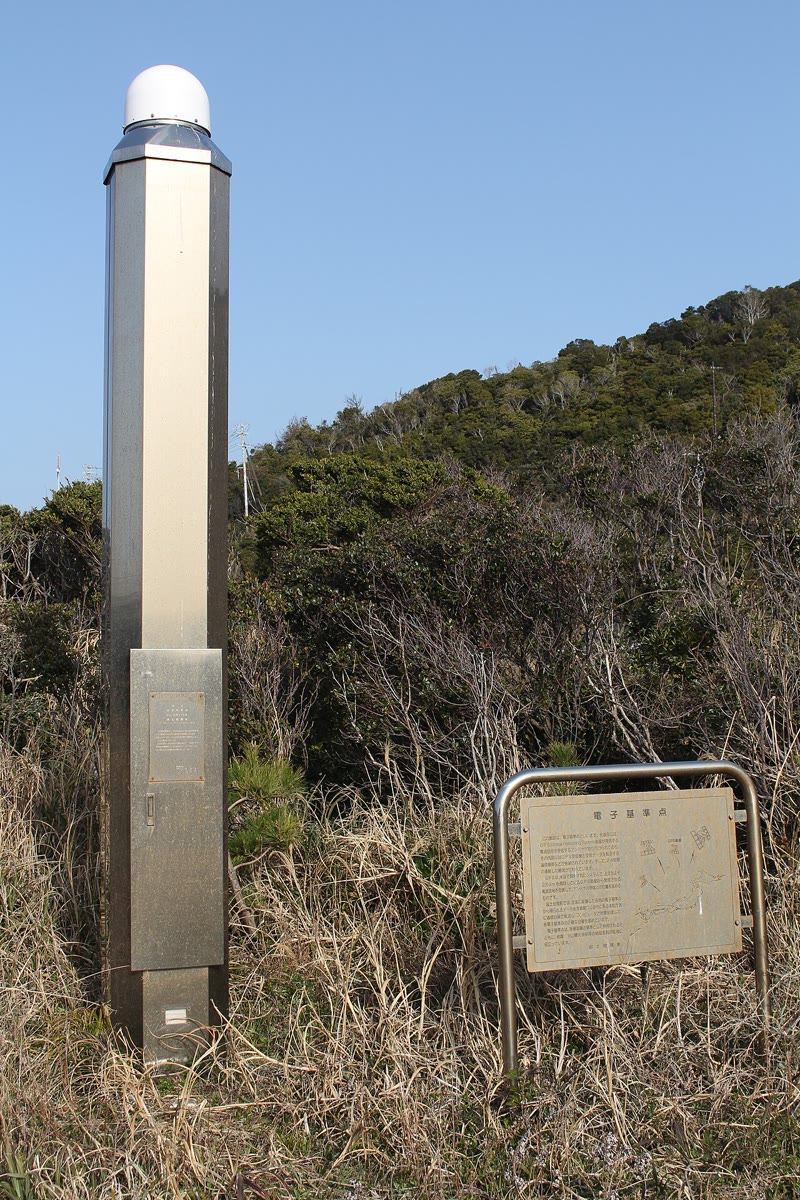
\includegraphics[width=\linewidth]{images/book3/b1-gnss-station.jpg}

{\scriptsize Uma estação permanente no Japão, com sua antena sob a cúpula
(Alpsdake, CC BY-SA 4.0).}
\end{minipage}
\end{inthefield}

As velocidades de estações nos interiores de duas placas dão um \omterm{def:b1:plate-kinematics:euler-pole}{vetor de Euler}
próprio, independente do registro geológico. Para a Eurásia em relação à
América do Norte, tal vetor prevê \qty{17.0}{mm.yr^{-1}} na Islândia, cerca de
\qty{8}{\percent} menos que os \qty{18.6}{mm.yr^{-1}} médios em
\qty{3.16}{Myr} (figura acima). A corda entre Reykjavik e Stavanger, ambas
em partes estáveis de suas placas, alonga-se \qty{17.5}{mm.yr^{-1}}; o
vetor de satélite prevê \qty{17.1}{mm.yr^{-1}}, o geológico
\qty{18.6}{mm.yr^{-1}}. Através do Atlântico Norte, uma taxa medida em algumas
décadas e uma taxa média de três milhões de anos concordam, portanto, a menos de um
décimo: ali, as placas se movem hoje quase como se moveram por milhões de
anos.
% ledger: morvel:gps-eu-na, morvel:eu-na, ngl:reyk, ngl:stas (chord rates computed in calc/ch12.py)

Dentro da zona de fronteira o quadro é menos simples, pois as estações se movem com
mais que as placas. Mais de um décimo da Islândia está sob calotas de gelo, e
a maioria delas vem perdendo massa desde cerca de 1890: a \omterm{def:b1:layered-earth:layers}{crosta} sob elas sobe à medida que
a carga diminui, e se move horizontalmente afastando-se do gelo que afina. A
estação de Höfn, na costa sudeste perto da maior calota, sobe
\qty{12.9}{mm.yr^{-1}}.
% ledger: spaans:iceland-gia, ngl:hofn

\section{Exercícios}

Tome $R = \qty{6371}{km}$ em todos os exercícios.

\begin{exercise}[$\star$]\label{exo:b1:plate-kinematics:1}
O \omterm{def:b1:plate-kinematics:euler-pole}{vetor de Euler} da Eurásia em relação à América do Norte tem a taxa
\qty{0.210}{\degree\per\Myr}. (a) Converta-a para \unit{rad.yr^{-1}} e para
\unit{rad.s^{-1}}. (b) Quanto tempo levaria uma volta completa? (c) Calcule $\omega R$ em
\unit{mm.yr^{-1}}.
% ledger: morvel:eu-na
\end{exercise}

\begin{exercise}[$\star$]\label{exo:b1:plate-kinematics:2}
Com o mesmo \omterm{def:b1:plate-kinematics:euler-pole}{vetor de Euler}, calcule a velocidade relativa das duas placas a
\ang{30}, \ang{60} e \ang{90} do \omterm{def:b1:plate-kinematics:euler-pole}{polo de Euler}. Onde ao longo da fronteira
de placas o espalhamento seria mais rápido?
\end{exercise}

\begin{exercise}[$\star$]\label{exo:b1:plate-kinematics:3}
O subcron normal Jaramillo durou de \qty{1.072}{Ma} a \qty{0.988}{Ma}.
(a) Qual a largura da listra que ele forma em cada flanco de uma dorsal com uma
\omterm{def:b1:plate-kinematics:spreading-rate}{taxa de espalhamento de metade} de \qty{50}{mm.yr^{-1}}? E de \qty{10}{mm.yr^{-1}}? (b) Qual é a
largura total da listra do cron normal atual, que começou
\qty{0.781}{Ma}, em uma dorsal com taxa de metade de \qty{10}{mm.yr^{-1}}?
% ledger: iodp:gpts2004
\end{exercise}

\begin{exercise}[$\star$]\label{exo:b1:plate-kinematics:4}
Em um perfil atravessando uma dorsal, a borda jovem da anomalia do cron C2An,
com \qty{2.581}{Ma}, fica a \qty{66}{km} a oeste do eixo e a \qty{64}{km} a leste
dele. Calcule as duas \omterm{def:b1:plate-kinematics:spreading-rate}{taxas de espalhamento de metade} e a \omterm{def:b1:plate-kinematics:spreading-rate}{taxa de espalhamento completa}. O
espalhamento é simétrico?
% ledger: iodp:gpts2004
\end{exercise}

\begin{exercise}[$\star\star$]\label{exo:b1:plate-kinematics:5}
Um ponto da dorsal de Gakkel, no oceano Ártico, fica a \ang{85}\,N, \ang{0}\,L.
Calcule sua distância angular ao \omterm{def:b1:plate-kinematics:euler-pole}{polo de Euler} Eurásia--América do Norte
(\ang{61.8}\,N, \ang{139.6}\,L, \qty{0.210}{\degree\per\Myr}) e a taxa de espalhamento
ali. Compare com as taxas medidas de \qtyrange{11}{12}{mm.yr^{-1}}.
% ledger: morvel:eu-na
\end{exercise}

\begin{exercise}[$\star\star$]\label{exo:b1:plate-kinematics:6}
Na \omterm{def:b1:plate-kinematics:triple-junction}{junção tripla} dos Açores, \ang{39.44}\,N, \ang{29.83}\,W, calcule (a) a distância angular ao \omterm{def:b1:plate-kinematics:euler-pole}{polo de Euler} Eurásia--América do Norte, (b) a taxa de espalhamento,
e (c) o \omterm{def:b1:spherical-astronomy:horizontal}{azimute} do movimento relativo. (d) Que \omterm{def:b1:geological-maps:attitude}{direção} você prevê para as falhas transformantes da dorsal logo ao norte da junção?
% ledger: morvel:eu-na, morvel:azores
\end{exercise}

\begin{exercise}[$\star\star$]\label{exo:b1:plate-kinematics:7}
(a) Escreva os \omterm{def:b1:plate-kinematics:euler-pole}{vetores de Euler} $\vec\omega_{\mathrm{EU\,NA}}$ (\ang{61.8}\,N,
\ang{139.6}\,L, \qty{0.210}{\degree\per\Myr}) e $\vec\omega_{\mathrm{NB\,NA}}$
(\ang{79.2}\,N, \ang{40.2}\,L, \qty{0.233}{\degree\per\Myr}) em componentes cartesianas, em \unit{\degree\per\Myr}. (b) Deduza $\vec\omega_{\mathrm{NB\,EU}}$,
seu polo e sua taxa. (c) Por que esta é a melhor maneira de conhecer o movimento da Núbia em relação à Eurásia?
% ledger: morvel:eu-na, morvel:nb-na
\end{exercise}

\begin{exercise}[$\star\star$]\label{exo:b1:plate-kinematics:8}
Seja $\vec e_x$ apontando para \ang{0}\,N, \ang{0}\,L, $\vec e_y$ para \ang{0}\,N,
\ang{90}\,L e $\vec e_z$ para o polo norte. Com a fórmula de Rodrigues, calcule
a imagem de $\vec e_x$ (a) pela rotação de \ang{90} em torno de $\vec e_z$
seguida pela rotação de \ang{90} em torno de $\vec e_x$; (b) pelas mesmas duas
rotações na ordem oposta. (c) O que isso significa para a reconstrução das posições passadas de uma placa?
\end{exercise}

\begin{exercise}[$\star\star$]\label{exo:b1:plate-kinematics:9}
Três placas A, B e C se encontram em uma junção dorsal--dorsal--dorsal. Em relação a A,
a placa B se move a \qty{30}{mm.yr^{-1}} para leste e a placa C a
\qty{40}{mm.yr^{-1}} para o sul. (a) Desenhe o triângulo de velocidades.
(b) Calcule a velocidade e o \omterm{def:b1:spherical-astronomy:horizontal}{azimute} de C em relação a B. (c) Qual é a direção da
dorsal entre B e C se ela se espalha perpendicularmente ao seu eixo?
\end{exercise}

\begin{exercise}[$\star\star\star$]\label{exo:b1:plate-kinematics:10}
(a) Mostre que o traço da matriz $R$ de uma rotação de $\alpha$ em torno de um eixo
qualquer é $1 + 2\cos\alpha$. (b) A matriz
\[
  R = \begin{pmatrix} 0 & 0 & 1\\ 1 & 0 & 0\\ 0 & 1 & 0\end{pmatrix}
\]
é ortogonal com determinante $1$. Encontre seu eixo, como \omterm{def:b1:spherical-astronomy:geographic}{latitude} e \omterm{def:b1:spherical-astronomy:geographic}{longitude},
e seu ângulo. (c) Confira sua resposta aplicando $R$ a $\vec e_x$, $\vec e_y$
e $\vec e_z$.
\end{exercise}

\begin{exercise}[$\star\star\star$]\label{exo:b1:plate-kinematics:11}
Antes do posicionamento por satélite, os \omterm{def:b1:plate-kinematics:euler-pole}{polos de Euler} eram encontrados a partir das direções das
falhas transformantes. (a) Mostre que o \omterm{def:b1:plate-kinematics:euler-pole}{polo de Euler} está sobre o \omterm{def:b1:spherical-astronomy:spherical-triangle}{círculo máximo} que passa por um ponto de uma falha transformante e é perpendicular à falha ali, e que o polo fica portanto na direção de $\vec t_1\times\vec t_2$, onde $\vec t_1$ e
$\vec t_2$ são vetores unitários ao longo de duas falhas transformantes de uma mesma fronteira.
(b) As falhas transformantes têm \omterm{def:b1:geological-maps:attitude}{direção} de \ang{95} perto da \omterm{def:b1:plate-kinematics:triple-junction}{junção tripla} dos Açores
(\ang{39.44}\,N, \ang{29.83}\,W) e de \ang{103} na Islândia (\ang{64.5}\,N,
\ang{18}\,W). O vetor horizontal unitário na \omterm{def:b1:spherical-astronomy:geographic}{latitude} $\varphi$ e \omterm{def:b1:spherical-astronomy:geographic}{longitude}
$\lambda$ apontando para o \omterm{def:b1:spherical-astronomy:horizontal}{azimute} $\beta$ é $\sin\beta\,\vec e +
\cos\beta\,\vec n$, com $\vec e = (-\sin\lambda, \cos\lambda, 0)$ e $\vec n =
(-\sin\varphi\cos\lambda, -\sin\varphi\sin\lambda, \cos\varphi)$. Localize o
polo. (c) Quão bem duas transformantes determinam o polo?
% ledger: morvel:eu-na
\end{exercise}

\begin{exercise}[$\star\star\star$]\label{exo:b1:plate-kinematics:12}
A posição leste de uma estação, a cada três meses durante três anos, é
(em milímetros, a partir de $t = 0$):
\begin{center}\small
\begin{tabular}{l*{13}{c}}
\hline
$t$ (yr) & 0 & 0.25 & 0.5 & 0.75 & 1 & 1.25 & 1.5 & 1.75 & 2 & 2.25 & 2.5 & 2.75 & 3\\
$x$ (mm) & 4 & 5 & 6 & 15 & 24 & 25 & 26 & 65 & 74 & 75 & 76 & 85 & 94\\
\hline
\end{tabular}
\end{center}
É composta de um movimento estacionário, uma oscilação sazonal e um salto causado por um
terremoto. (a) Calcule a velocidade a partir das primeiras e últimas posições.
(b) Calcule as nove diferenças entre posições separadas exatamente por um ano, e
sua mediana. (c) Explique por que a mediana das diferenças de um ano é uma
estimativa robusta da velocidade estacionária, e quando ela falharia.
\end{exercise}

\section{Problema: a Islândia se separa}

\begin{problem}[{Problema de fim de semana --- a abertura do Atlântico Norte através da
Islândia, medida de três maneiras}]
\label{pb:b1:plate-kinematics:1}
% values: calc/ch12.py (Part II profile invented for the problem; real Euler
% vectors, chron ages and station velocities)
% ledger: morvel:eu-na, morvel:nb-na, iodp:gpts2004, ngl:reyk, ngl:stas, ngl:hofn
A Islândia está sobre a Dorsal Meso-Atlântica, entre a placa norte-americana, a oeste,
e a placa euroasiática, a leste. Tome $R = \qty{6371}{km}$ e, para a Eurásia em
relação à América do Norte, o \omterm{def:b1:plate-kinematics:euler-pole}{vetor de Euler} com seu polo em
\ang{61.8}\,N, \ang{139.6}\,L e a taxa \qty{0.210}{\degree\per\Myr}.

\medskip
\noindent\textbf{Parte I --- O vetor da placa.}
\begin{enumerate}
  \item Converta a taxa para \unit{rad.yr^{-1}} e calcule $\omega R$ em
        \unit{mm.yr^{-1}}.
  \item Calcule a distância angular $\Delta$ do polo ao centro da
        Islândia, \ang{64.5}\,N, \ang{18}\,W.
  \item Deduza a \omterm{def:b1:plate-kinematics:spreading-rate}{taxa de espalhamento completa} através da Islândia prevista pelo
        vetor da placa.
  \item Calcule o \omterm{def:b1:spherical-astronomy:horizontal}{azimute} do polo visto da Islândia, e o \omterm{def:b1:spherical-astronomy:horizontal}{azimute} do
        movimento da Eurásia em relação à América do Norte.
  \item Decomponha essa velocidade em suas componentes para leste e para norte.
  \item Na dorsal de Gakkel, a \ang{86}\,N, \ang{60}\,L, que taxa o mesmo
        vetor dá? Por que a fronteira ali é tão mais lenta?
\end{enumerate}

\noindent\textbf{Parte II --- As listras magnéticas.}
Um perfil magnético de navio atravessando a dorsal de Reykjanes, a sudoeste da Islândia, perto de
\ang{63}\,N, \ang{23}\,W, percorrido na direção do espalhamento, dá as seguintes
distâncias do eixo a três limites de cron (um perfil construído para
este problema):
\begin{center}\small
\begin{tabular}{lccc}
\hline
limite & idade (Ma) & a oeste do eixo (km) & a leste do eixo (km)\\
\hline
base de C1n & 0.781 & 9.7 & 10.1\\
borda jovem de C2An & 2.581 & 26.8 & 27.3\\
borda jovem de C5n & 9.779 & 94 & 97\\
\hline
\end{tabular}
\end{center}
\begin{enumerate}[resume]
  \item A partir da borda jovem de C5n, calcule as duas \omterm{def:b1:plate-kinematics:spreading-rate}{taxas de espalhamento de metade}.
  \item Deduza a \omterm{def:b1:plate-kinematics:spreading-rate}{taxa de espalhamento completa} desde \qty{9.8}{Ma}.
  \item Calcule também a taxa completa a partir das duas fronteiras mais jovens. As
        três concordam? Descreva como elas mudam com a idade do limite.
  \item O espalhamento é simétrico? A assimetria muda a taxa completa?
  \item Na dorsal de Reykjanes, os limites entre listras são deslocados para longe do eixo em \qty{5.0}{km} ao todo, somando os dois flancos.
        Corrija as três taxas completas. Por que a correção importou mais para o limite mais jovem?
  \item Qual é a largura da listra do subcron Jaramillo
        (\qtyrange{1.072}{0.988}{Ma}) em cada flanco, com a taxa de metade corrigida? Compare com o deslocamento da questão 11. A anomalia Jaramillo é, mesmo assim, claramente reconhecida nos perfis da dorsal de Reykjanes, mas está ausente na dorsal de Gakkel: o que isso sugere?
  \item O vetor da placa prevê \qty{19.0}{mm.yr^{-1}} no perfil. Compare
        com suas taxas corrigidas.
\end{enumerate}

\noindent\textbf{Parte III --- Os satélites.}
As estações permanentes REYK (Reykjavik, \ang{64.139}\,N, \ang{21.955}\,W) e
STAS (Stavanger, \ang{59.018}\,N, \ang{5.599}\,L) estão sobre as placas norte-americana e
euroasiática. Suas velocidades medidas fazem a corda entre elas alongar-se
em \qty{17.5}{mm.yr^{-1}}.
\begin{enumerate}[resume]
  \item Calcule a distância angular entre as duas estações, e o comprimento
        da corda.
  \item Quanto tempo a corda leva para alongar-se um metro?
  \item O vetor da placa dá a STAS uma velocidade de \qty{18.9}{mm.yr^{-1}} em direção a
        \ang{114.8} em relação à América do Norte. O \omterm{def:b1:spherical-astronomy:spherical-triangle}{círculo máximo} de REYK
        chega a STAS seguindo em direção a \ang{123.1}. Calcule a componente da velocidade ao longo desta direção, e então o alongamento previsto da
        corda, que faz o ângulo $\Delta/2$ com a horizontal em STAS.
  \item Compare o alongamento medido com o previsto. O que poderia explicar a
        diferença?
  \item Em relação à América do Norte, REYK se move a \qty{1.07}{mm.yr^{-1}} para o oeste e \qty{0.97}{mm.yr^{-1}} para o sul, e a estação HOFN (Höfn,
        sudeste da Islândia) a \qty{21.12}{mm.yr^{-1}} para o leste e
        \qty{6.97}{mm.yr^{-1}} para o sul. Calcule a velocidade e o \omterm{def:b1:spherical-astronomy:horizontal}{azimute} de HOFN
        em relação a REYK.
  \item Compare com a Parte I. HOFN também sobe \qty{12.9}{mm.yr^{-1}}. Por que as
        estações dentro da Islândia são uma má medida do movimento da placa?
\end{enumerate}

\noindent\textbf{Parte IV --- Dez milhões de anos, e a junção ao sul.}
\begin{enumerate}[resume]
  \item Em \qty{10}{Myr}, de que ângulo a Eurásia gira em torno do polo em relação à
        América do Norte?
  \item A que distância percorre, nesse tempo, um ponto da Eurásia no meio da Islândia ao longo de seu pequeno círculo? Compare com a largura corrigida da \omterm{def:b1:layered-earth:layers}{crosta} formada desde a borda jovem de C5n na Parte II.
  \item Na \omterm{def:b1:plate-kinematics:triple-junction}{junção tripla} dos Açores, os vetores de placa dão à Eurásia
        \qty{22.9}{mm.yr^{-1}} em direção a \ang{95.1} e à Núbia
        \qty{19.2}{mm.yr^{-1}} em direção a \ang{103.8}, ambos em relação à
        América do Norte. Calcule a velocidade da Eurásia em relação à Núbia.
  \item Esta junção é \omterm{def:b1:plate-kinematics:triple-junction}{estável}? Que tipo de fronteira a velocidade da
        questão 22 implica entre a Eurásia e a Núbia?
  \item Reúna as taxas de abertura das Partes I, II e III. Quais concordam, e qual método mede o movimento das placas no menor intervalo de tempo?
  \item Com aproximação de um milímetro por ano, que \omterm{def:b1:plate-kinematics:spreading-rate}{taxa de espalhamento completa} através da Islândia dão ao mesmo tempo o vetor da placa e as listras magnéticas corrigidas?
\end{enumerate}
\end{problem}
